\documentclass{standalone}
\usepackage{tikz}
\usetikzlibrary{patterns, positioning}
\usepackage[sfdefault]{ClearSans} %% option 'sfdefault' activates Clear Sans as the default text font
\usepackage[T1]{fontenc}

\begin{document}
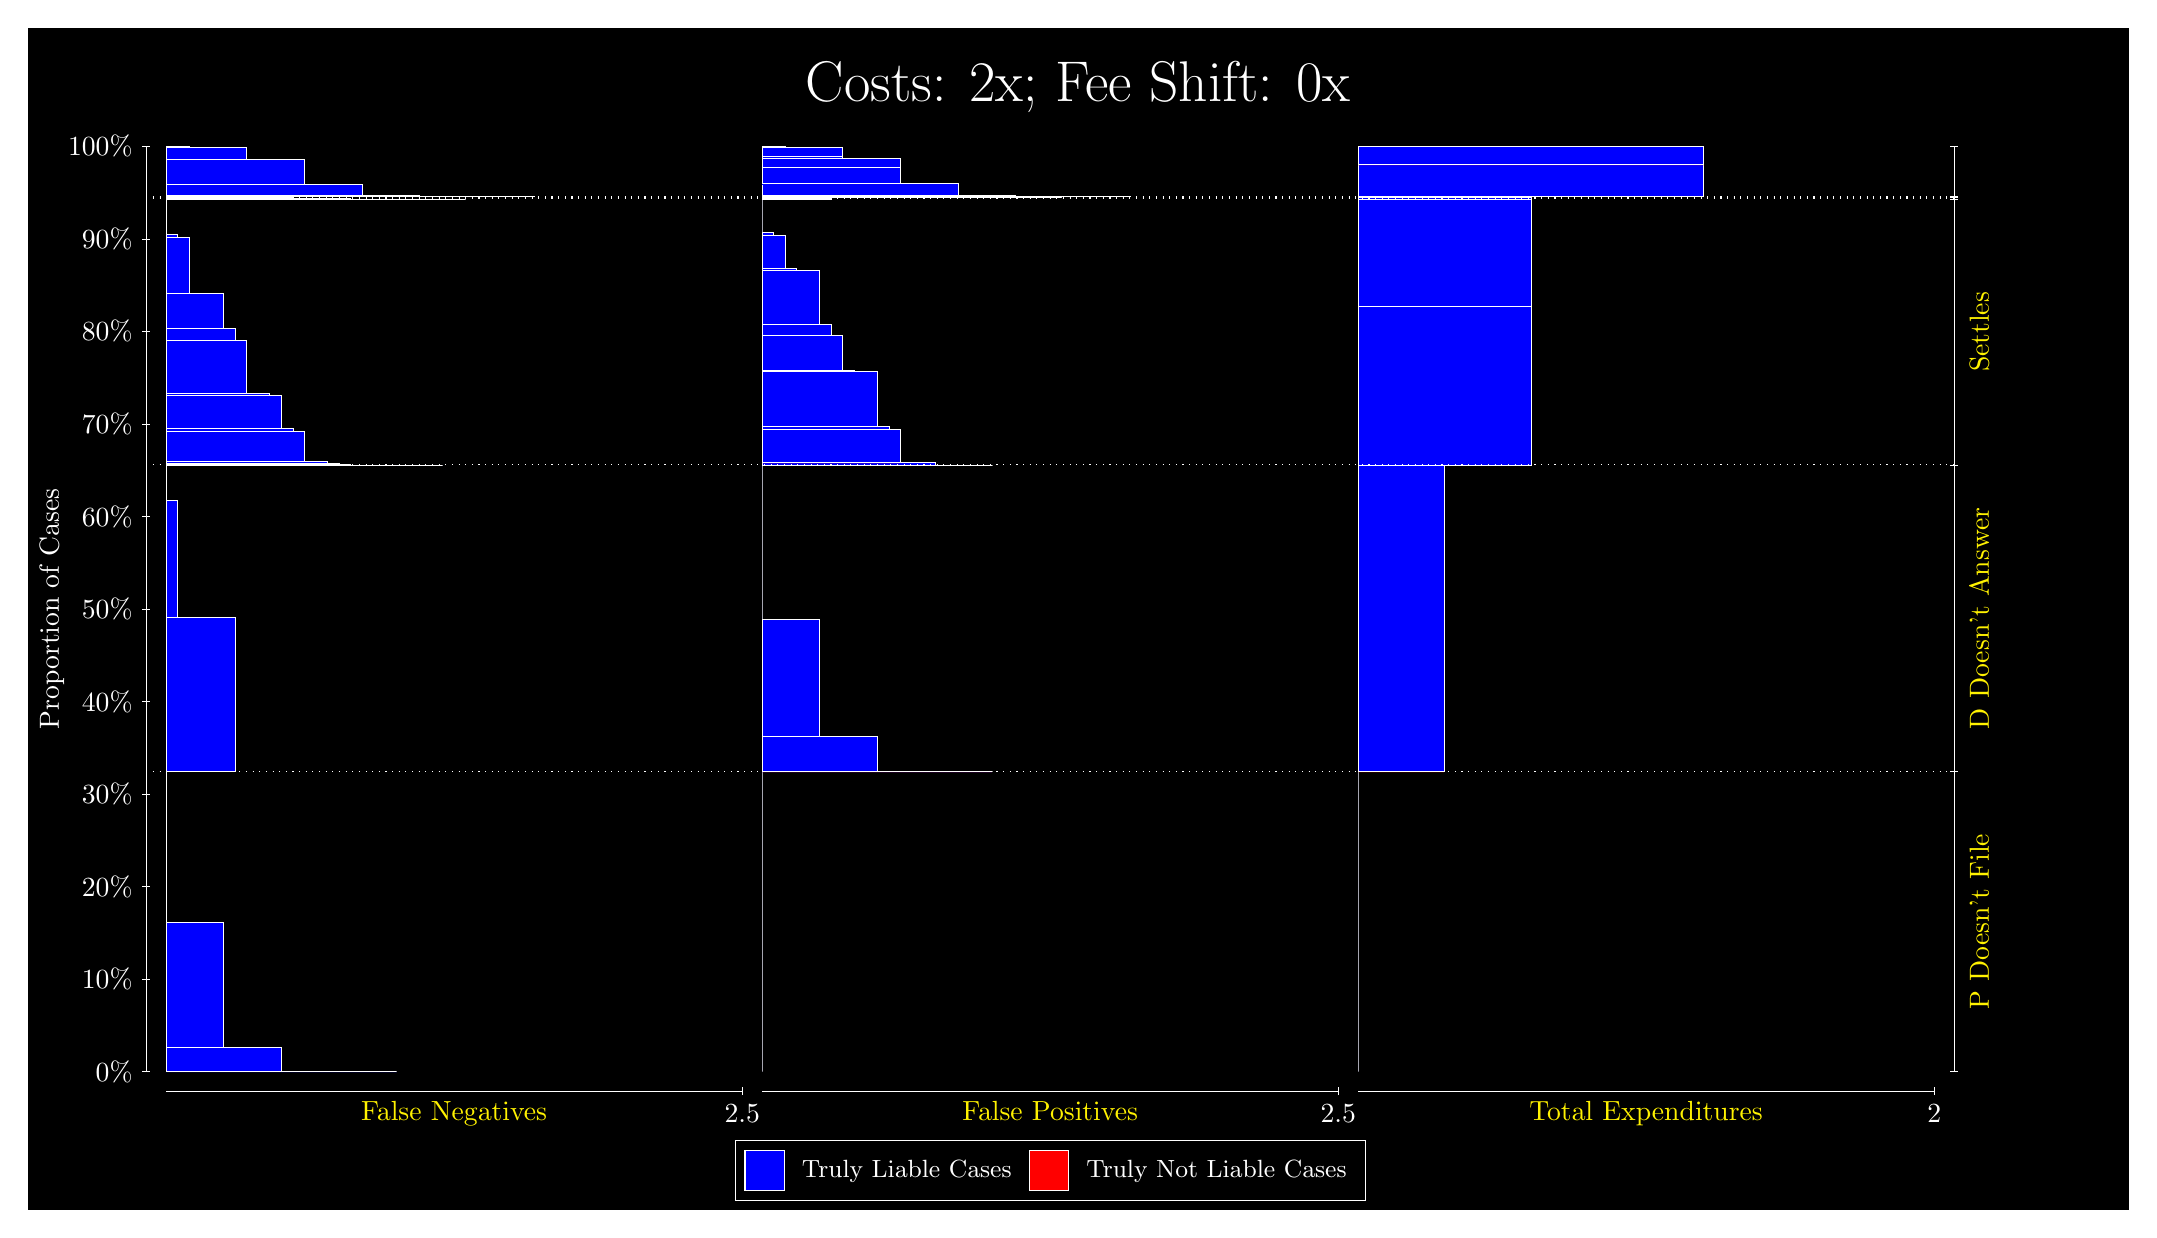
\begin{tikzpicture}
\draw[fill=black] (0,0) rectangle (26.667,15);
\draw[text=white] (0,13.5) rectangle (26.667,15) node[midway] {\huge Costs: 2x; Fee Shift: 0x};
\draw[white, very thin] (1.5,1.75) -- (1.5,13.5);
\node[rotate=90, text=white, anchor=center] at (0.3, 7.625) {Proportion of Cases};
\draw[white, very thin] (1.45,1.75) -- (1.55,1.75);
\node[text=white, anchor=east] at (1.45, 1.75) {0\%};
\draw[white, very thin] (1.45,2.925) -- (1.55,2.925);
\node[text=white, anchor=east] at (1.45, 2.925) {10\%};
\draw[white, very thin] (1.45,4.1) -- (1.55,4.1);
\node[text=white, anchor=east] at (1.45, 4.1) {20\%};
\draw[white, very thin] (1.45,5.275) -- (1.55,5.275);
\node[text=white, anchor=east] at (1.45, 5.275) {30\%};
\draw[white, very thin] (1.45,6.45) -- (1.55,6.45);
\node[text=white, anchor=east] at (1.45, 6.45) {40\%};
\draw[white, very thin] (1.45,7.625) -- (1.55,7.625);
\node[text=white, anchor=east] at (1.45, 7.625) {50\%};
\draw[white, very thin] (1.45,8.8) -- (1.55,8.8);
\node[text=white, anchor=east] at (1.45, 8.8) {60\%};
\draw[white, very thin] (1.45,9.975) -- (1.55,9.975);
\node[text=white, anchor=east] at (1.45, 9.975) {70\%};
\draw[white, very thin] (1.45,11.15) -- (1.55,11.15);
\node[text=white, anchor=east] at (1.45, 11.15) {80\%};
\draw[white, very thin] (1.45,12.325) -- (1.55,12.325);
\node[text=white, anchor=east] at (1.45, 12.325) {90\%};
\draw[white, very thin] (1.45,13.5) -- (1.55,13.5);
\node[text=white, anchor=east] at (1.45, 13.5) {100\%};

\draw[white, very thin] (24.457,1.75) -- (24.457,13.5);
\draw[white, very thin] (24.407,1.75) -- (24.507,1.75);
\node[anchor=west] at (24.407, 1.75) {};
\draw[white, very thin] (24.407,5.5572) -- (24.507,5.5572);
\node[anchor=west] at (24.407, 5.5572) {};
\draw[white, very thin] (24.407,9.4543) -- (24.507,9.4543);
\node[anchor=west] at (24.407, 9.4543) {};
\draw[white, very thin] (24.407,12.833) -- (24.507,12.833);
\node[anchor=west] at (24.407, 12.833) {};
\draw[white, very thin] (24.407,12.854) -- (24.507,12.854);
\node[anchor=west] at (24.407, 12.854) {};
\draw[white, very thin] (24.407,12.868) -- (24.507,12.868);
\node[anchor=west] at (24.407, 12.868) {};
\draw[white, very thin] (24.407,13.5) -- (24.507,13.5);
\node[anchor=west] at (24.407, 13.5) {};

\draw[white, very thin, fill=blue] (1.75,1.75) rectangle (4.6775,1.75);
\draw[white, very thin, fill=blue] (1.75,1.75) rectangle (3.9457,1.7525);
\draw[white, very thin, fill=blue] (1.75,1.7525) rectangle (3.2138,2.0519);
\draw[white, very thin, fill=blue] (1.75,2.0519) rectangle (2.4819,3.6444);
\draw[white, very thin, fill=red] (1.75,3.6444) rectangle (1.75,3.6444);
\draw[white, very thin, fill=blue] (1.75,3.6444) rectangle (1.75,5.5572);
\draw[white, very thin, fill=blue] (1.75,5.5572) rectangle (2.6283,7.5134);
\draw[white, very thin, fill=blue] (1.75,7.5134) rectangle (1.8964,9.0065);
\draw[white, very thin, fill=red] (1.75,9.0065) rectangle (1.75,9.0065);
\draw[white, very thin, fill=blue] (1.75,9.0065) rectangle (1.75,9.4543);
\draw[white, very thin, fill=blue] (1.75,9.4543) rectangle (5.2631,9.4543);
\draw[white, very thin, fill=blue] (1.75,9.4543) rectangle (4.6775,9.4543);
\draw[white, very thin, fill=blue] (1.75,9.4543) rectangle (4.5312,9.4548);
\draw[white, very thin, fill=blue] (1.75,9.4548) rectangle (4.092,9.4558);
\draw[white, very thin, fill=blue] (1.75,9.4558) rectangle (3.9457,9.4719);
\draw[white, very thin, fill=blue] (1.75,9.4719) rectangle (3.7993,9.4949);
\draw[white, very thin, fill=blue] (1.75,9.4949) rectangle (3.5065,9.8805);
\draw[white, very thin, fill=blue] (1.75,9.8805) rectangle (3.3602,9.9188);
\draw[white, very thin, fill=blue] (1.75,9.9188) rectangle (3.2138,10.342);
\draw[white, very thin, fill=blue] (1.75,10.342) rectangle (3.0674,10.36);
\draw[white, very thin, fill=blue] (1.75,10.36) rectangle (2.7746,11.042);
\draw[white, very thin, fill=blue] (1.75,11.042) rectangle (2.6283,11.185);
\draw[white, very thin, fill=blue] (1.75,11.185) rectangle (2.4819,11.638);
\draw[white, very thin, fill=blue] (1.75,11.638) rectangle (2.3355,11.638);
\draw[white, very thin, fill=blue] (1.75,11.638) rectangle (2.0428,12.342);
\draw[white, very thin, fill=blue] (1.75,12.342) rectangle (1.8964,12.378);
\draw[white, very thin, fill=red] (1.75,12.378) rectangle (1.75,12.378);
\draw[white, very thin, fill=blue] (1.75,12.378) rectangle (1.75,12.833);
\draw[white, very thin, fill=blue] (1.75,12.833) rectangle (5.5558,12.833);
\draw[white, very thin, fill=blue] (1.75,12.833) rectangle (4.8239,12.833);
\draw[white, very thin, fill=blue] (1.75,12.833) rectangle (4.092,12.835);
\draw[white, very thin, fill=blue] (1.75,12.835) rectangle (3.3602,12.848);
\draw[white, very thin, fill=blue] (1.75,12.848) rectangle (2.6283,12.854);
\draw[white, very thin, fill=red] (1.75,12.854) rectangle (1.75,12.854);
\draw[white, very thin, fill=blue] (1.75,12.854) rectangle (2.6283,12.86);
\draw[white, very thin, fill=blue] (1.75,12.86) rectangle (1.8964,12.868);
\draw[white, very thin, fill=red] (1.75,12.868) rectangle (1.75,12.868);
\draw[white, very thin, fill=blue] (1.75,12.868) rectangle (1.75,12.868);
\draw[white, very thin, fill=blue] (1.75,12.868) rectangle (6.4341,12.868);
\draw[white, very thin, fill=blue] (1.75,12.868) rectangle (5.7022,12.868);
\draw[white, very thin, fill=blue] (1.75,12.868) rectangle (4.9703,12.878);
\draw[white, very thin, fill=blue] (1.75,12.878) rectangle (4.2384,13.024);
\draw[white, very thin, fill=blue] (1.75,13.024) rectangle (3.5065,13.341);
\draw[white, very thin, fill=blue] (1.75,13.341) rectangle (2.7746,13.488);
\draw[white, very thin, fill=blue] (1.75,13.488) rectangle (2.0428,13.5);
\draw[white, very thin, fill=red] (1.75,13.5) rectangle (1.75,13.5);
\draw[white, very thin, fill=blue] (1.75,13.5) rectangle (1.75,13.5);
\draw[white, very thin, fill=red] (9.3189,1.75) rectangle (9.3189,1.75);
\draw[white, very thin, fill=blue] (9.3189,1.75) rectangle (9.3189,5.5572);
\draw[white, very thin, fill=red] (9.3189,5.5572) rectangle (12.246,5.5572);
\draw[white, very thin, fill=blue] (9.3189,5.5572) rectangle (12.246,5.5572);
\draw[white, very thin, fill=blue] (9.3189,5.5572) rectangle (11.515,5.5672);
\draw[white, very thin, fill=blue] (9.3189,5.5672) rectangle (10.783,6.0051);
\draw[white, very thin, fill=blue] (9.3189,6.0051) rectangle (10.051,7.4982);
\draw[white, very thin, fill=blue] (9.3189,7.4982) rectangle (9.3189,9.4543);
\draw[white, very thin, fill=red] (9.3189,9.4543) rectangle (12.246,9.4543);
\draw[white, very thin, fill=blue] (9.3189,9.4543) rectangle (12.246,9.4543);
\draw[white, very thin, fill=red] (9.3189,9.4543) rectangle (11.661,9.4543);
\draw[white, very thin, fill=blue] (9.3189,9.4543) rectangle (11.661,9.4552);
\draw[white, very thin, fill=blue] (9.3189,9.4552) rectangle (11.515,9.4821);
\draw[white, very thin, fill=red] (9.3189,9.4821) rectangle (11.075,9.4821);
\draw[white, very thin, fill=blue] (9.3189,9.4821) rectangle (11.075,9.9094);
\draw[white, very thin, fill=blue] (9.3189,9.9094) rectangle (10.929,9.9455);
\draw[white, very thin, fill=blue] (9.3189,9.9455) rectangle (10.783,10.649);
\draw[white, very thin, fill=red] (9.3189,10.649) rectangle (10.49,10.649);
\draw[white, very thin, fill=blue] (9.3189,10.649) rectangle (10.49,10.65);
\draw[white, very thin, fill=blue] (9.3189,10.65) rectangle (10.344,11.103);
\draw[white, very thin, fill=blue] (9.3189,11.103) rectangle (10.197,11.246);
\draw[white, very thin, fill=blue] (9.3189,11.246) rectangle (10.051,11.928);
\draw[white, very thin, fill=blue] (9.3189,11.928) rectangle (9.758,11.945);
\draw[white, very thin, fill=blue] (9.3189,11.945) rectangle (9.6116,12.369);
\draw[white, very thin, fill=blue] (9.3189,12.369) rectangle (9.4652,12.407);
\draw[white, very thin, fill=blue] (9.3189,12.407) rectangle (9.3189,12.833);
\draw[white, very thin, fill=red] (9.3189,12.833) rectangle (10.197,12.833);
\draw[white, very thin, fill=blue] (9.3189,12.833) rectangle (10.197,12.839);
\draw[white, very thin, fill=blue] (9.3189,12.839) rectangle (9.4652,12.853);
\draw[white, very thin, fill=blue] (9.3189,12.853) rectangle (9.3189,12.854);
\draw[white, very thin, fill=red] (9.3189,12.854) rectangle (13.125,12.854);
\draw[white, very thin, fill=blue] (9.3189,12.854) rectangle (13.125,12.854);
\draw[white, very thin, fill=blue] (9.3189,12.854) rectangle (12.393,12.854);
\draw[white, very thin, fill=blue] (9.3189,12.854) rectangle (11.661,12.854);
\draw[white, very thin, fill=blue] (9.3189,12.854) rectangle (10.929,12.863);
\draw[white, very thin, fill=blue] (9.3189,12.863) rectangle (10.197,12.868);
\draw[white, very thin, fill=red] (9.3189,12.868) rectangle (14.003,12.868);
\draw[white, very thin, fill=blue] (9.3189,12.868) rectangle (14.003,12.868);
\draw[white, very thin, fill=red] (9.3189,12.868) rectangle (13.271,12.868);
\draw[white, very thin, fill=blue] (9.3189,12.868) rectangle (13.271,12.868);
\draw[white, very thin, fill=red] (9.3189,12.868) rectangle (12.539,12.868);
\draw[white, very thin, fill=blue] (9.3189,12.868) rectangle (12.539,12.88);
\draw[white, very thin, fill=blue] (9.3189,12.88) rectangle (11.807,13.026);
\draw[white, very thin, fill=red] (9.3189,13.026) rectangle (11.807,13.026);
\draw[white, very thin, fill=blue] (9.3189,13.026) rectangle (11.807,13.027);
\draw[white, very thin, fill=blue] (9.3189,13.027) rectangle (11.075,13.24);
\draw[white, very thin, fill=red] (9.3189,13.24) rectangle (11.075,13.24);
\draw[white, very thin, fill=blue] (9.3189,13.24) rectangle (11.075,13.344);
\draw[white, very thin, fill=blue] (9.3189,13.344) rectangle (10.344,13.37);
\draw[white, very thin, fill=blue] (9.3189,13.37) rectangle (10.344,13.49);
\draw[white, very thin, fill=blue] (9.3189,13.49) rectangle (9.6116,13.49);
\draw[white, very thin, fill=blue] (9.3189,13.49) rectangle (9.6116,13.5);
\draw[white, very thin, fill=blue] (9.3189,13.5) rectangle (9.3189,13.5);
\draw[white, very thin, fill=red] (16.888,1.75) rectangle (16.888,1.75);
\draw[white, very thin, fill=blue] (16.888,1.75) rectangle (16.888,5.5572);
\draw[white, very thin, fill=red] (16.888,5.5572) rectangle (17.986,5.5572);
\draw[white, very thin, fill=blue] (16.888,5.5572) rectangle (17.986,9.4543);
\draw[white, very thin, fill=red] (16.888,9.4543) rectangle (19.083,9.4543);
\draw[white, very thin, fill=blue] (16.888,9.4543) rectangle (19.083,11.472);
\draw[white, very thin, fill=red] (16.888,11.472) rectangle (19.083,11.472);
\draw[white, very thin, fill=blue] (16.888,11.472) rectangle (19.083,12.833);
\draw[white, very thin, fill=red] (16.888,12.833) rectangle (19.083,12.833);
\draw[white, very thin, fill=blue] (16.888,12.833) rectangle (19.083,12.854);
\draw[white, very thin, fill=red] (16.888,12.854) rectangle (19.083,12.854);
\draw[white, very thin, fill=blue] (16.888,12.854) rectangle (19.083,12.868);
\draw[white, very thin, fill=red] (16.888,12.868) rectangle (21.279,12.868);
\draw[white, very thin, fill=blue] (16.888,12.868) rectangle (21.279,13.266);
\draw[white, very thin, fill=red] (16.888,13.266) rectangle (21.279,13.266);
\draw[white, very thin, fill=blue] (16.888,13.266) rectangle (21.279,13.5);
\draw[white, dotted] (1.5,5.5572) -- (24.457,5.5572);
\draw[white, dotted] (1.5,9.4543) -- (24.457,9.4543);
\draw[white, dotted] (1.5,12.833) -- (24.457,12.833);
\draw[white, dotted] (1.5,12.854) -- (24.457,12.854);
\draw[white, dotted] (1.5,12.868) -- (24.457,12.868);
\draw[white, very thin] (1.75,1.5) -- (9.0689,1.5);
\node[text=yellow, anchor=north] at (5.4094, 1.5) {False Negatives};
\draw[white, very thin] (9.0689,1.45) -- (9.0689,1.55);
\node[text=white, anchor=north] at (9.0689, 1.45) {2.5};

\draw[white, very thin] (9.3189,1.5) -- (16.638,1.5);
\node[text=yellow, anchor=north] at (12.978, 1.5) {False Positives};
\draw[white, very thin] (16.638,1.45) -- (16.638,1.55);
\node[text=white, anchor=north] at (16.638, 1.45) {2.5};

\draw[white, very thin] (16.888,1.5) -- (24.207,1.5);
\node[text=yellow, anchor=north] at (20.547, 1.5) {Total Expenditures};
\draw[white, very thin] (24.207,1.45) -- (24.207,1.55);
\node[text=white, anchor=north] at (24.207, 1.45) {2};

\node[text=yellow, centered, rotate=90] at (24.777, 3.6536) {P Doesn't File};
\node[text=yellow, centered, rotate=90] at (24.777, 7.5058) {D Doesn't Answer};
\node[text=yellow, centered, rotate=90] at (24.777, 11.144) {Settles};




\draw (12.978300999999998,1.5) node[draw=none] (baseCoordinate) {};
\begin{scope}[align=center]
        \matrix[scale=0.5, draw=white, below=0.5cm of baseCoordinate, nodes={draw}, column sep=0.1cm]{
            \node[rectangle, draw, minimum width=0.5cm, minimum height=0.5cm, fill=blue] {}; &
            \node[draw=none, font=\small, text=white] (B) {Truly Liable Cases}; &
            \node[rectangle, draw, minimum width=0.5cm, minimum height=0.5cm, fill=red] {}; &
            \node[draw=none, font=\small, text=white] (B) {Truly Not Liable Cases}; \\
            };
\end{scope}

\end{tikzpicture}
\end{document}